\section{Experiments}
\label{sec:exp}

\subsection{Datasets}
\label{sec:datasets}

We evaluate on six public battery degradation datasets spanning
different chemistries, capacities, and degradation behaviors
(Table~\ref{tab:datasets}): CALCE (LCO, rated 1.1\,Ah), NASA
\cite{ref_nasa_data} (LCO, 2.0\,Ah), MIT/Stanford \cite{ref_severson}
(LFP, 124 cells), PANASONIC (NCA, 3.03\,Ah), TJU (NCM+NCA,
2.5\,Ah), and GOTION (LFP large-format, 27\,Ah). End-of-life (EOL) thresholds follow rated
capacity times convention: 70\% for small cells and 80\% for
large-format cells. For MIT we use a 10-cell subset (8 training, 2 test) for this study.
All models use pure capacity input; internal resistance is used only
as an auxiliary input of the physics-extension rate head
(Section~\ref{sec:physics}).

\begin{table}[htbp]
\centering
\caption{Dataset overview.}
\label{tab:datasets}
\tiny
\begin{tabular}{lcccccl}
\toprule
Dataset & Chemistry & Rated & Cells & EOL (Ah) & Role \\
\midrule
CALCE & LCO & 1.1 Ah & 4 & 0.77 & primary, physics (IR) \\
NASA & LCO & 2.0 Ah & 4 & 1.40 & short-history \\
MIT & LFP & 1.07 Ah & 10* & 0.86 & cross-battery \\
PANASONIC & NCA & 3.03 Ah & 3 & 2.12 & regeneration \\
TJU & NCM+NCA & 2.5 Ah & 3 & 1.75 & long-cycle \\
GOTION & LFP (large-format) & 27 Ah & 3 & 21.60 & large-format fleet \\
\bottomrule
\end{tabular}
\end{table}

\subsection{Evaluation protocol}
\label{sec:protocol}

Following the standard protocol in PatchFormer \cite{ref_patchformer}
and RUL-Mamba \cite{ref_rulmamba}, we report trajectory
metrics per starting point (SP): R\textsuperscript{2}, MAE (mean absolute error),
RMSE (root mean squared error), and AE. Let TRUL be the true
remaining useful life in cycles at an SP (cycles from the SP to the
true EOL crossing), PRUL is the predicted RUL from the first threshold
crossing of the predicted capacity sequence, AE $= |\text{TRUL} -
\text{PRUL}|$ is the absolute RUL error in cycles, and RE $=$
AE/TRUL is the relative RUL error.

\emph{Training configuration.} All models use Adam (learning rate
$1\times10^{-3}$, batch size 64) for 100 epochs with a window of
$W{=}64$ cycles ($W{=}30$ for NASA, PANASONIC and GOTION, matching the
window convention of the baseline literature). These settings were
fixed during the ablation stage and held constant across datasets,
seeds, and model variants: no per-dataset or per-variant tuning is
applied to the reported results, so every variant compared in
Sections~\ref{sec:ablation}--\ref{sec:phys} shares the same optimizer
budget. We do not claim these configurations are optimal; a
sensitivity note is included in Section~\ref{sec:limitations}.
The main results (Table~\ref{tab:tableA}) additionally follow the
per-SP training protocol of PatchFormer. For each combination of dataset, prediction Start Point (SP), 
and random seed, a separate model with randomly initialized weights is trained from scratch, 
with no pre-trained weights or cross-set parameter reuse allowed. We use ten seeds per
SP (1--10), so each table cell aggregates ten independently trained
models. The ablation studies (Section~\ref{sec:ablation}) use the
same optimizer budget with ten seeds. The physics extension is
reported over the same ten seeds for its head, extrapolation, and
robustness studies, and the uncertainty study uses the ten-seed
full-data training described above (coverage
$93.5\%\pm0.9\%$).

\subsection{Main results}
\label{sec:main}

Figure~\ref{fig:traj} shows representative SOH trajectories with
sliding-window single-step predictions for one cell of each dataset;
Table~\ref{tab:tableA} reports the full per-SP results. The six datasets span distinct degradation regimes 
and operational scenarios. We present each as a standalone case study in the sections below: 
each case concludes with a discussion of the practical implications of our experimental results, 
as well as a benchmark comparison against state-of-the-art (SOTA) results reported on the same dataset.

\begin{figure*}[!t]
\centering
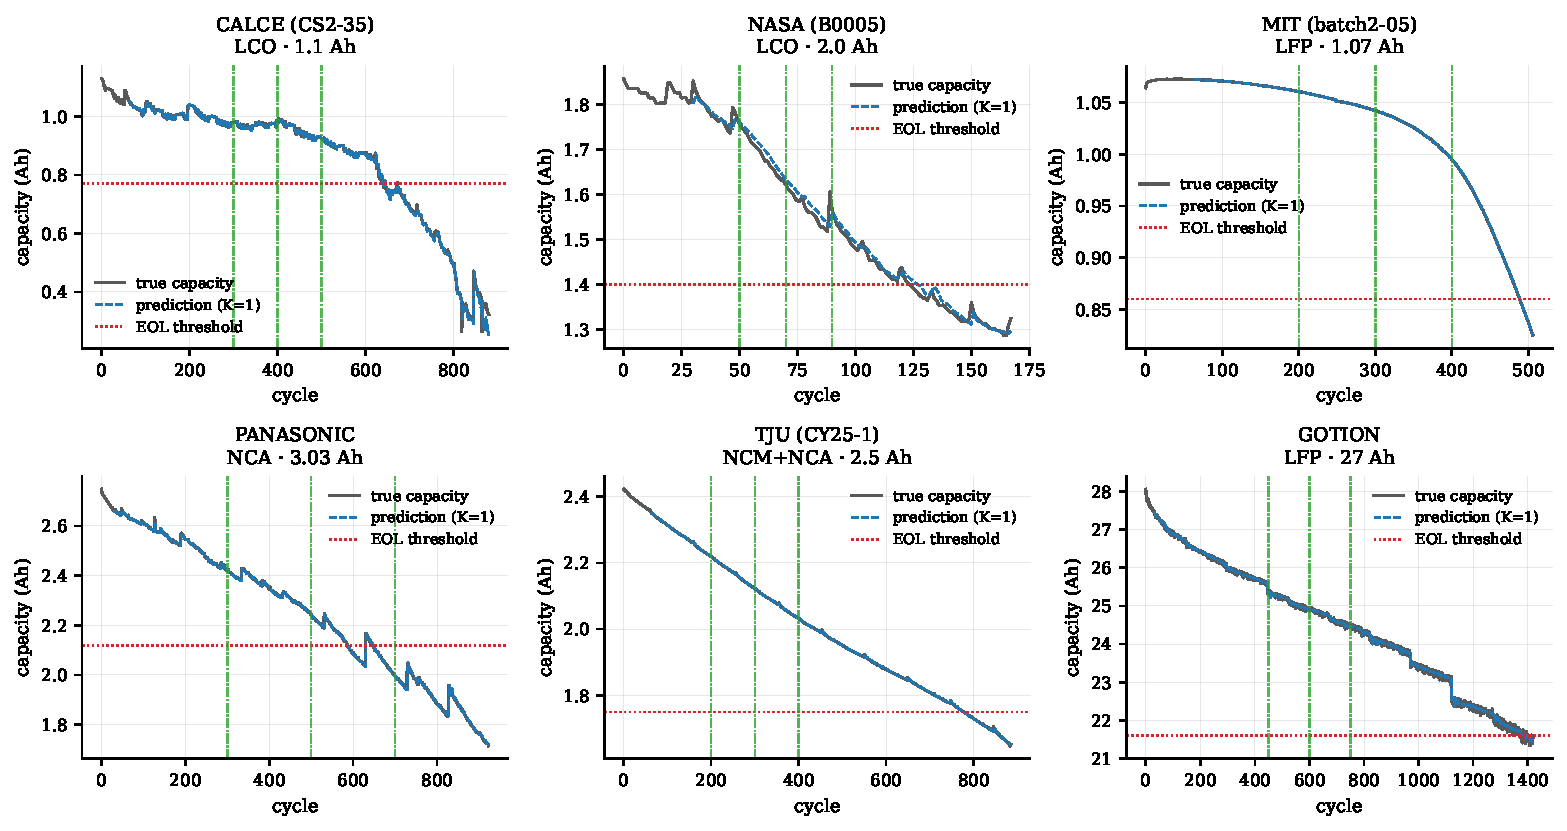
\includegraphics[width=\textwidth]{figures/fig_traj}
\caption{Single-step capacity prediction on one test cell per
dataset. Green dashed lines mark the starting points (SPs); red
dotted lines mark the EOL thresholds.}
\label{fig:traj}
\end{figure*}


Figure~\ref{fig:compare} shows our model ranks first (mean per-SP MAE) on PANASONIC, TJU, GOTION and MIT,
and second on NASA and CALCE — top-2 on all six datasets and
ahead of every generic time-series transformer.

\begin{figure*}[!t]
\centering
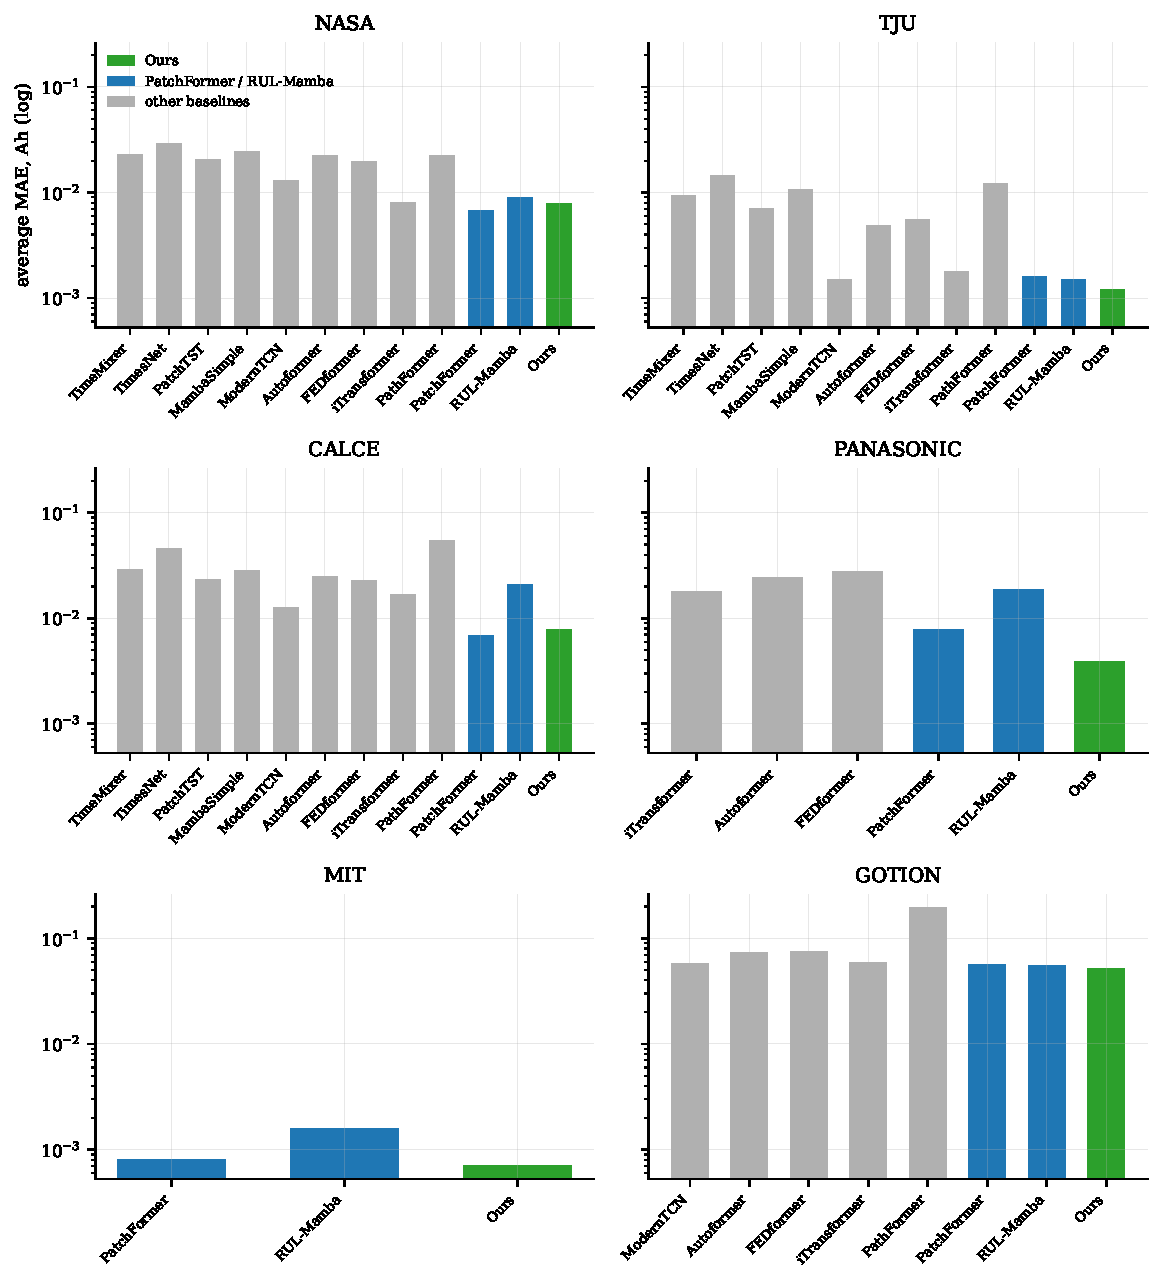
\includegraphics[width=\textwidth]{figures/fig_compare}
\caption{Per-SP trajectory MAE of the compared methods on all six
datasets, averaged over the three SPs (log scale). Green: Ours; blue:
PatchFormer/RUL-Mamba; gray: other baselines.}
\label{fig:compare}
\end{figure*}

\begin{table}[htbp]
\centering
\caption{Per-SP trajectory results, mean $\pm$ std
over ten seeds (1--10) per SP under the PatchFormer-consistent
per-SP protocol (a fresh model per (SP, seed)).}
\label{tab:tableA}
\scriptsize
\setlength{\tabcolsep}{1pt}
\begin{tabular}{lr rrrrr}
\toprule
Dataset & SP & TRUL & MAE & RMSE & R\textsuperscript{2} & AE \\
\midrule
CALCE & 300 & 339 & 0.0065$\pm$0.0007 & 0.0145$\pm$0.0013 & 0.9951$\pm$0.0008 & 3.2 \\
  & 400 & 239 & 0.0077$\pm$0.0010 & 0.0169$\pm$0.0019 & 0.9933$\pm$0.0015 & 2.5 \\
  & 500 & 139 & 0.0091$\pm$0.0016 & 0.0194$\pm$0.0028 & 0.9898$\pm$0.0030 & 2.4 \\
NASA & 50 & 73 & 0.0086$\pm$0.0016 & 0.0128$\pm$0.0011 & 0.9908$\pm$0.0018 & 0.9 \\
  & 70 & 53 & 0.0078$\pm$0.0008 & 0.0130$\pm$0.0004 & 0.9822$\pm$0.0011 & 0.4 \\
  & 90 & 33 & 0.0071$\pm$0.0008 & 0.0101$\pm$0.0010 & 0.9804$\pm$0.0036 & 0.5 \\
PANASONIC & 300 & 287 & 0.0038$\pm$0.0003 & 0.0098$\pm$0.0001 & 0.9976$\pm$0.0001 & 0.8 \\
  & 400 & 187 & 0.0037$\pm$0.0002 & 0.0103$\pm$0.0001 & 0.9965$\pm$0.0001 & 0.8 \\
  & 500 & 87 & 0.0041$\pm$0.0003 & 0.0113$\pm$0.0003 & 0.9936$\pm$0.0003 & 0.9 \\
TJU & 200 & 577 & 0.0010$\pm$0.0002 & 0.0015$\pm$0.0001 & 0.9999$\pm$0.0000 & 0.2 \\
  & 300 & 477 & 0.0011$\pm$0.0002 & 0.0016$\pm$0.0002 & 0.9998$\pm$0.0000 & 0.9 \\
  & 400 & 377 & 0.0014$\pm$0.0003 & 0.0020$\pm$0.0004 & 0.9996$\pm$0.0001 & 1.6 \\
MIT & 200 & 406 & 0.0005$\pm$0.0002 & 0.0008$\pm$0.0003 & 0.9998$\pm$0.0002 & 0.9 \\
  & 300 & 306 & 0.0007$\pm$0.0002 & 0.0009$\pm$0.0004 & 0.9997$\pm$0.0004 & 0.9 \\
  & 400 & 206 & 0.0008$\pm$0.0004 & 0.0010$\pm$0.0004 & 0.9995$\pm$0.0004 & 1.1 \\
GOTION & 450 & 921 & 0.0473$\pm$0.0006 & 0.0645$\pm$0.0013 & 0.9970$\pm$0.0001 & 18.2 \\
  & 600 & 771 & 0.0518$\pm$0.0019 & 0.0697$\pm$0.0026 & 0.9958$\pm$0.0003 & 10.7 \\
  & 750 & 621 & 0.0550$\pm$0.0006 & 0.0735$\pm$0.0019 & 0.9938$\pm$0.0003 & 15.1 \\
\midrule
\multicolumn{7}{l}{\emph{Average across all SPs and seeds: AE = 3.4 cycles, R\textsuperscript{2} = 0.9947.}} \\
\bottomrule
\end{tabular}
\end{table}

\begin{table*}[!t]
\centering
\caption{Comparison with reference baselines on all six
published-comparison datasets. MAE in Ah; each
dataset's starting points are listed under its name; bold marks the
best value in each column, ties are both bold. MambaSimple is the plain
Mamba model of \cite{ref_mamba}. Ours: means over ten
seeds (per-SP protocol), AE reported as mean over seeds; the two
self-run baselines (PatchFormer, RUL-Mamba) use ten repeats per SP.
$^{\ast}$The EOL cycle is the first crossing of the measured series; for
GOTION this is cycle~1371. The series oscillates across the threshold nine
times between cycles 1371 and 1415, so the reference is not sharply defined
and the AE reflects that ambiguity rather than model error. The unparenthesised
AE is measured against cycle~1371; the value in parentheses against
cycle~1391, obtained by locating both the measured series and the predicted
trajectory on a moving average. The cited baselines reference cycle~1392, so
their AE values are on the latter basis.}
\label{tab:lit_all}
\scriptsize
\setlength{\tabcolsep}{4pt}
\begin{tabular}{@{}ll rrr rrr rrr@{}}
\toprule
 & & \multicolumn{3}{c}{SP1} & \multicolumn{3}{c}{SP2} & \multicolumn{3}{c}{SP3} \\
\cmidrule(lr){3-5}\cmidrule(lr){6-8}\cmidrule(lr){9-11}
Dataset & Method & MAE & R\textsuperscript{2} & AE & MAE & R\textsuperscript{2} & AE & MAE & R\textsuperscript{2} & AE \\
\midrule
\multirow{6}{*}{\shortstack[l]{PANASONIC\\\emph{300/400/500}}} & PatchFormer & \textbf{0.0033} &\textbf{0.9977}&1.0& \textbf{0.0037} &\textbf{0.9965}&1.0& 0.0167 &0.9698&3.6 \\
  & RUL-Mamba & 0.0174 &0.9725&2.3& 0.0182 &0.9563&2.0& 0.0212 &0.9183&2.0 \\
  & iTransformer & 0.0162 &0.9790&1.2& 0.0175 &0.9654&1.2& 0.0203 &0.9278&1.4 \\
  & Autoformer & 0.0231 &0.9737&2.6& 0.0241 &0.9585&3.8& 0.0263 &0.9258&7.2 \\
  & FEDformer & 0.0257 &0.9648&6.8& 0.0269 &0.9446&6.8& 0.0295 &0.8896&8.4 \\
  & Ours &0.0038&0.9976&\textbf{0.8}&\textbf{0.0037}&\textbf{0.9965}&\textbf{0.8}&\textbf{0.0041}&\textbf{0.9936}&\textbf{0.9} \\
\midrule
\multirow{12}{*}{\shortstack[l]{TJU\\\emph{200/300/400}}} & TimeMixer & 0.0071 &0.9963&7.6& 0.0086 &0.9919&6.0& 0.0123 &0.9777&6.5 \\
  & TimesNet & 0.0163 &0.9830&1.0& 0.0146 &0.9808&\textbf{0.2}& 0.0130 &0.9783&\textbf{0.4} \\
  & PatchTST & 0.0078 &0.9960&9.8& 0.0069 &0.9952&7.4& 0.0067 &0.9925&5.8 \\
  & MambaSimple & 0.0119 &0.9902&9.5& 0.0107 &0.9887&7.7& 0.0094 &0.9874&5.5 \\
  & ModernTCN & 0.0014 &0.9998&2.8& 0.0015 &0.9997&2.7& 0.0016 &0.9995&2.7 \\
  & Autoformer & 0.0050 &0.9979&5.5& 0.0049 &0.9970&5.4& 0.0047 &0.9957&4.8 \\
  & FEDformer & 0.0058 &0.9977&6.0& 0.0056 &0.9968&5.7& 0.0054 &0.9954&4.9 \\
  & iTransformer & 0.0017 &0.9998&1.8& 0.0018 &0.9996&1.8& 0.0019 &0.9994&1.4 \\
  & PathFormer & 0.0100 &0.9930&9.9& 0.0112 &0.9855&12.1& 0.0152 &0.9606&15.6 \\
  & PatchFormer & 0.0014 &0.9998&2.1& 0.0015 &0.9997&2.2& 0.0019 &0.9994&3.0 \\
  & RUL-Mamba & 0.0014 &0.9998&2.8& 0.0015 &0.9997&2.9& 0.0016 &0.9995&2.9 \\
  & Ours &\textbf{0.0010}&\textbf{0.9999}&\textbf{0.2}&\textbf{0.0011}&\textbf{0.9998}&0.9&\textbf{0.0014}&\textbf{0.9996}&1.6 \\
\midrule
\multirow{8}{*}{\shortstack[l]{GOTION\\\emph{450/600/750}}} & ModernTCN & 0.0553 &0.9960&\textbf{8.3}& 0.0570 &0.9947&\textbf{8.0}& 0.0619 &0.9921&\textbf{7.8} \\
  & Autoformer & 0.0694 &0.9930&9.9& 0.0716 &0.9909&9.4& 0.0783 &0.9864&8.8 \\
  & FEDformer & 0.0720 &0.9922&10.5& 0.0733 &0.9902&10.1& 0.0794 &0.9857&9.5 \\
  & iTransformer & 0.0564 &0.9957&9.8& 0.0586 &0.9944&9.5& 0.0642 &0.9913&9.0 \\
  & PathFormer & 0.1663 &0.9276&12.8& 0.1925 &0.8797&15.2& 0.2306 &0.7766&16.7 \\
  & PatchFormer & 0.0536 &0.9964&9.6& 0.0563 &0.9952&9.1& 0.0606 &0.9928&8.0 \\
  & RUL-Mamba & 0.0525 &0.9960&15.2& 0.0552 &0.9946&15.9& 0.0598 &0.9917&15.7 \\
  & Ours &\textbf{0.0473}&\textbf{0.9970}&18.2\;(1.7)&\textbf{0.0518}&\textbf{0.9958}&10.7\;(2.6)&\textbf{0.0550}&\textbf{0.9938}&15.1\;(2.6) \\
\midrule
\multirow{3}{*}{\shortstack[l]{MIT\\\emph{200/300/400}}} & PatchFormer & 0.0008 &0.9997&\textbf{0.6}& 0.0008 &\textbf{0.9997}&\textbf{0.8}& 0.0009 &\textbf{0.9995}&\textbf{0.4} \\
  & RUL-Mamba & 0.0011 &0.9994&1.4& 0.0016 &0.9991&1.1& 0.0022 &0.9979&1.0 \\
  & Ours &\textbf{0.0005}&\textbf{0.9998}&0.9&\textbf{0.0007}&\textbf{0.9997}&0.9&\textbf{0.0008}&\textbf{0.9995}&1.1 \\
\midrule
\multirow{12}{*}{\shortstack[l]{NASA\\\emph{50/70/90}}} & TimeMixer & 0.0239 &0.9540&8.0& 0.0241 &0.9014&6.7& 0.0203 &0.8290&9.0 \\
  & TimesNet & 0.0364 &0.8753&3.0& 0.0298 &0.8349&2.9& 0.0213 &0.8699&3.0 \\
  & PatchTST & 0.0260 &0.9405&4.2& 0.0201 &0.9333&3.9& 0.0150 &0.9209&5.0 \\
  & MambaSimple & 0.0301 &0.9254&6.7& 0.0250 &0.9034&5.7& 0.0188 &0.8943&4.1 \\
  & ModernTCN & 0.0166 &0.9750&2.9& 0.0127 &0.9700&4.4& 0.0098 &0.9483&6.8 \\
  & Autoformer & 0.0234 &0.9341&3.6& 0.0230 &0.8721&4.1& 0.0213 &0.8153&4.2 \\
  & FEDformer & 0.0215 &0.9569&4.7& 0.0199 &0.9217&5.0& 0.0172 &0.8961&5.8 \\
  & iTransformer & 0.0076 &0.9891&5.4& 0.0078 &0.9772&4.3& 0.0086 &0.9528&4.5 \\
  & PathFormer & 0.0274 &0.9228&5.1& 0.0214 &0.9100&5.6& 0.0186 &0.8941&7.9 \\
  & PatchFormer & \textbf{0.0061} &\textbf{0.9919}&\textbf{0.2}& \textbf{0.0072} &0.9808&1.4& 0.0072 &0.9623&2.5 \\
  & RUL-Mamba & 0.0089 &0.9889&1.7& 0.0090 &0.9771&1.3& 0.0091 &0.9568&1.8 \\
  & Ours &0.0086&0.9908&0.9&0.0078&\textbf{0.9822}&\textbf{0.4}&\textbf{0.0071}&\textbf{0.9804}&\textbf{0.5} \\
\midrule
\multirow{12}{*}{\shortstack[l]{CALCE\\\emph{300/400/500}}} & TimeMixer & 0.0244 &0.9608&15.8& 0.0287 &0.9512&16.4& 0.0341 &0.9245&16.7 \\
  & TimesNet & 0.0369 &0.9469&42.0& 0.0456 &0.9304&44.3& 0.0559 &0.8938&47.0 \\
  & PatchTST & 0.0200 &0.9750&9.5& 0.0230 &0.9683&11.4& 0.0276 &0.9497&11.5 \\
  & MambaSimple & 0.0239 &0.9682&15.8& 0.0281 &0.9607&18.6& 0.0333 &0.9416&19.9 \\
  & ModernTCN & 0.0109 &0.9909&3.2& 0.0124 &0.9888&3.3& 0.0147 &0.9838&5.3 \\
  & Autoformer & 0.0216 &0.9738&10.3& 0.0242 &0.9681&11.0& 0.0281 &0.9550&12.0 \\
  & FEDformer & 0.0197 &0.9782&14.4& 0.0224 &0.9735&15.9& 0.0260 &0.9628&17.6 \\
  & iTransformer & 0.0141 &0.9880&6.9& 0.0166 &0.9849&8.1& 0.0198 &0.9787&10.9 \\
  & PathFormer & 0.0431 &0.9060&40.3& 0.0532 &0.8814&41.9& 0.0659 &0.8212&43.4 \\
  & RUL-Mamba & 0.0175 &0.9782&11.5& 0.0201 &0.9733&13.1& 0.0245 &0.9605&15.7 \\
  & PatchFormer & \textbf{0.0057} &\textbf{0.9962}&\textbf{0.9}& \textbf{0.0068} &\textbf{0.9951}&\textbf{0.9}& \textbf{0.0081} &\textbf{0.9930}&\textbf{1.0} \\
  & Ours &0.0065&0.9951&3.2&0.0077&0.9933&2.5&0.0091&0.9898&2.4 \\
\midrule
\bottomrule
\end{tabular}
\end{table*}

\subsubsection{PANASONIC: regeneration-rich fleet operation}
PANASONIC (NCA, 3.03\,Ah) is the regeneration benchmark: staircase
profiles with local capacity recoveries. Our model ranks first on the
mean per-SP MAE (Table~\ref{tab:lit_all}: $0.0039$, against $0.0079$
for the closest method, an official-repo reproduction of PatchFormer,
and $0.0162$ for the strongest published baseline at SP300). That
reproduction is ahead at one start point only, SP300 (MAE $0.0033$
vs.\ $0.0038$, $p<10^{-3}$ over ten repeats); at SP400 the two are
indistinguishable ($p=0.12$) and ours leads SP500 by $\sim$4$\times$
(MAE $0.0041$ vs.\ $0.0167$). Figure~\ref{fig:regen}
shows why the free-head readout tracks a $0.024$\,Ah local rise
without overshoot, while a structurally monotonic predictor cannot
represent this pattern at all. In practice, real
fleet data is non-monotonic. A model with a structural monotonicity
bias would systematically mis-schedule maintenance after recovery
events. The free head covers this regime, and the monotonic rate head
(Section~\ref{sec:physics}) is deliberately reserved for
monotonic-degradation cells: the two readouts partition the
degradation regimes by design.


\begin{figure*}[!t]
\centering
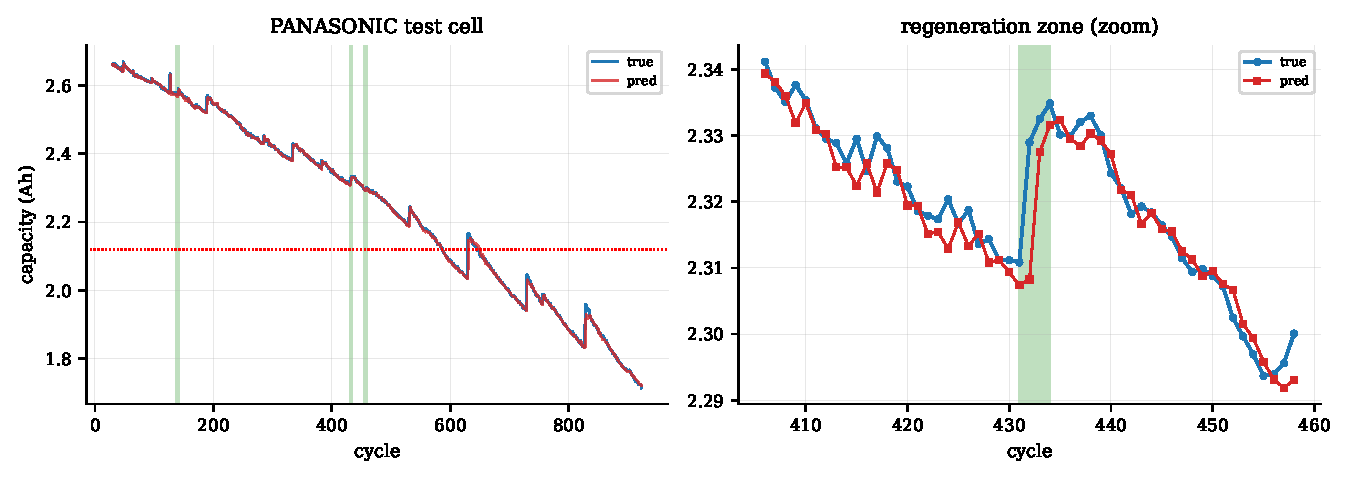
\includegraphics[width=\textwidth]{figures/fig_regen}
\caption{PANASONIC test cell: full trajectory (left, green bands mark
regeneration segments) and zoom on the strongest regeneration zone
(right). The free-head model tracks the local capacity rise without
overshoot; a structurally monotonic predictor cannot represent this
pattern at all.}
\label{fig:regen}
\end{figure*}


\subsubsection{TJU: long-life cycle counting}
TJU (NCM/NCA, 2.5\,Ah, $\sim$900-cycle cells) is the long-life,
low-noise regime. The model leads on MAE at every starting point
(Table~\ref{tab:lit_all}: $0.0010$, $0.0011$ and $0.0014$ against
$0.0014$, $0.0015$ and $0.0016$ for the closest baselines), and its
R\textsuperscript{2} and AE are best at SP400 as well ($0.9996$ vs.\
$0.9995$ and $1.6$ vs.\ $2.7$--$2.9$).
\emph{In practice:} long-life assets accumulate decisions
slowly; the combination of near-perfect trajectory fit and calibrated
intervals (Section~\ref{sec:conf}) supports low-frequency,
high-stakes replacement planning.





\subsubsection{GOTION: large-format fleet operation}
GOTION (LFP, 27\,Ah, three cells, 2 train / 1 test) is the
large-format regime: 1400-cycle deep-discharge profiles with a wide
dynamic range, the format of grid-storage and heavy-duty
applications. Our
model leads every reported and reproduced baseline on MAE at each SP
(Table~\ref{tab:lit_all}: $0.0473$-$0.0550$ against $0.0525$-$0.0598$
for the closest of them), and also leads their R\textsuperscript{2}
($0.9970$ vs.\ $0.9964$ at SP450); the margin over the reported
time-series baselines ranges from $1.2\times$ (ModernTCN) to
$4.2\times$ (PathFormer). The gap concentrates in the capacity-scale
normalization, where operating a 27\,Ah range reacts badly to
per-window statistics. Part of that spread comes from the EOL reference
itself: the measured series crosses the threshold nine times between cycles
1371 and 1415, and locating the reference on a smoothed series (cycle~1391,
matching the cited sources) lowers our AE to $1.7/2.6/2.6$ (footnote
$^{\ast}$ in Table~\ref{tab:lit_all}). The remainder is scale-dependent:
the 27\,Ah envelope spans
$6.7$\,Ah at $\sim$4.7\,mAh/cycle, so a given capacity error
converts to 4--10$\times$ more cycles than on the small-cell
datasets; relative error stays at 2--5\%. \emph{Operational
implication:} large-format assets are exactly where on-device
monitoring pays for itself in maintenance optics; the surplus
accuracy here translates into replacement planning with margin.





\subsubsection{MIT: cross-cell fleet screening}
MIT (LFP, 1.074\,Ah, 8 train / 2 test cells) is our large-scale
fleet proxy: many training cells, unseen test cells. Over the two
test cells the model achieves R$^2 \ge 0.9995$ at every SP
(Table~\ref{tab:tableA}), with mean AE $0.2$ cycles on one test cell
and $1.6$ on the other (10-seed means), exceeding the published MIT
result of Zhou et al.\ \cite{ref_zhou2025}
(R\textsuperscript{2} $0.9902$) under a different protocol (7-step multi-point).
Against the two self-run baselines on this dataset
(Table~\ref{tab:lit_all}) the model ranks first on both
MAE and R\textsuperscript{2} at all three starting points, and within one
cycle of the best AE. Per-SP protocol (every (SP, seed) retrained from scratch, 10 seeds
per SP) is applied uniformly. \emph{In practice:}
cross-cell generalization at R$^2 \approx 1$ is the enabler for
fleet-scale screening and grading with per-device confidence.


\subsubsection{NASA: short-history rapid assessment}
NASA (LCO, 2.0\,Ah, $\sim$168-cycle cells) is the shortest-history
scenario: new assets or limited telemetry. With only 168 cycles the
model still reaches R$^2 \ge 0.9804$ and mean AE $0.6$ cycles
(Table~\ref{tab:lit_all}); on R\textsuperscript{2} we exceed the self-run
PatchFormer result at SP90
($0.9804$ vs.\ $0.9623$) and at SP70 ($0.9822$ vs.\ $0.9808$), and at
SP90 it leads on MAE as well ($0.0071$ vs.\ $0.0072$; AE $0.5$ vs.\
$2.5$). PatchFormer stays ahead on MAE at SP50 and SP70.
\emph{In practice:}
short histories are the regime where rapid commissioning checks and
second-life screening must run with limited data; the model's
trajectory error is already small from $\sim$50 cycles of
observation.



\subsubsection{CALCE: long-term monotonic monitoring}
CALCE (LCO, 1.1\,Ah, four cells) exhibits smooth, monotonic fade over
$\sim$900 cycles, the canonical asset-monitoring regime. The model
ranks second only to PatchFormer on every reported metric among all
compared baselines (Table~\ref{tab:lit_all}: MAE
$0.0065$--$0.0091$ vs.\ $0.0057$--$0.0081$; R\textsuperscript{2} within $0.004$; AE
mean $2.4$--$3.2$ vs.\ $0.9$--$1.0$); the AE seed-to-seed spread
($1$--$7$ cycles, per-SP means $3.2$/$2.5$/$2.4$), comes from seeds
whose near-flat tail crossing
amplifies a small trajectory bias into several cycles of RUL error,
as quantified below. \emph{Operational
implication:} on
monotonic cells the free head is the workhorse for daily SOH
monitoring, while the monotonic rate head of Section~\ref{sec:physics}
applies with zero regeneration risk and improves MAE by 40\%.


\emph{On the CALCE AE spread.} The AE column deserves an
explicit note: across the ten seeds per SP the AE values span
1--7 at SP300 (mean 3.2), 1--7 at SP400 (mean 2.5) and 0--6 at
SP500 (mean 2.4), and the maximum is not a training failure but a
geometric property of the test cell. Near the EOL threshold the
CALCE trajectory is nearly flat (local slope $\approx 1.9$\,mAh/cycle),
so a local
prediction bias of $\sim$10\,mAh near the tail, diluted
to $\le 0.001$ in the full-segment MAE, shifts the threshold
crossing by 5--7 cycles.
The same mechanism keeps PatchFormer's CALCE AE in a narrow band
(0.9--1.0): on flat tails AE is a coarse-grained statistic; we report the
mean and flag the seed-to-seed spread explicitly. On CALCE, where we
additionally run PatchFormer's official code under our identical
protocol, the self-run baseline gives AE $=$ 0.9 at SP300 against our
AE $=$ 3.2 (R\textsuperscript{2} $0.9962$ vs.\ $0.9951$).

\subsection{Ablation studies}
\label{sec:ablation}

This section ablates the architecture only; the physics extension is
validated separately in Section~\ref{sec:phys}. The comparison is run
on PANASONIC, the regeneration-rich benchmark whose staircase profiles
stress the multi-scale design's intended regime, and it uses the same
per-SP protocol and ten seeds as the main results, so the two tables
are directly comparable.

The exchange is the only difference between the two configurations in
Table~\ref{tab:ablation}. Both are multi-scale, and both are grown to the
main model's parameter count ($484{,}067$ against $483{,}866$, a
$0.04\,\%$ gap), so the comparison isolates the cross-scale mechanism
rather than the $42\,\%$ parameter deficit that separates the ablated
model from the main one at its default width. Under the per-SP protocol
of the main results, the exchange lowers MAE at every starting point, by
$6.6\,\%$, $6.3\,\%$ and $4.4\,\%$, and does so significantly at the
first two (paired two-sided Wilcoxon over ten seeds, $p=0.020$ and
$p=0.027$) but not at SP500 ($p=0.375$). Because the three starting
points probe one claim rather than three independent ones, we also
average each seed over the three before testing: the exchange then wins
$22$ of the $30$ (starting point, seed) pairs ($p=0.008$, sign test)
with a $5.7\,\%$ mean reduction in MAE ($p=0.014$). The margin is
largest at the earliest starting point and smallest at the latest, which
is the ordering a cross-scale mechanism should show: it corrects a local
branch against the global trend, and the earlier the forecast begins the
more horizon that correction has to work over.
\begin{table}[htbp]
\centering
\caption{Architecture ablation on PANASONIC, under the per-SP protocol
of Table~\ref{tab:tableA}. Both arms are multi-scale and both are grown
to the main model's parameter count (no-exchange $484{,}067$,
stage-query $483{,}866$), so they differ only in the cross-scale
exchange. MAE in Ah, mean $\pm$ std over ten seeds per
starting point; bold marks the lower MAE. $p$ is the paired two-sided
Wilcoxon signed-rank over those ten seeds; the aggregate row averages
each seed over the three starting points before testing, so the claim is
tested once rather than three times.}
\label{tab:ablation}
\footnotesize
\setlength{\tabcolsep}{6pt}
\begin{tabular}{lccc}
\toprule
Starting point & multi, no exchange & multi + stage-query & $p$ \\
\midrule
300 & 0.0041$\pm$0.0004 & $\mathbf{0.0038\pm0.0003}$ & 0.020 \\
400 & 0.0039$\pm$0.0002 & $\mathbf{0.0037\pm0.0002}$ & 0.027 \\
500 & 0.0043$\pm$0.0004 & $\mathbf{0.0041\pm0.0003}$ & 0.375 \\
\midrule
\multicolumn{3}{l}{\emph{All three starting points, averaged per seed}} & \textbf{0.014} \\
\bottomrule
\end{tabular}
\end{table}

\subsection{Physics extension and interpretability}
\label{sec:phys}

We compared every physics injection route in the literature against
the main backbone: (i) an objective regularizer with an
Arrhenius-plus-IR rate prior; (ii) physics features concatenated to
the input ($[C,\mathrm{IR}]$ on CALCE; temperature and EIS
resistance $[C,T,\mathrm{Re},\mathrm{Rct}]$ on NASA); (iii) a
structural monotone head trained under the per-window z-score
protocol. All three fail: the regularizer's constant-rate prior
conflicts with the EOL acceleration tail ($R^2$ $0.61\to0.34$ on
extrapolation), the features are redundant with capacity history (no
gain in any setting), and the structural head cannot represent the
positive z-score targets of plateau segments (training loss stalls).
The surviving mechanism, the rate head of
Section~\ref{sec:physics}, moves the constraint to absolute
capacity space and to an independently measured feature; a control
free head trained in the same absolute space (MAE
$0.0089\pm0.0058$ over ten seeds, ranging $0.0052$--$0.0242$)
isolates the mechanism from the objective, and the rate head
itself improves CALCE MAE by 53\% ($0.00424\pm0.00002$ vs
$0.0089\pm0.0058$). Its value shows in the
two regimes where physics is expected to matter;
Figures~\ref{fig:extrap} and \ref{fig:robust} together with
Tables~\ref{tab:extrap} and \ref{tab:robust} quantify both, and we
close with the interpretability of the learned physics term.

\subsubsection{Unseen-tail extrapolation}

We train on the first $90\%$ of each cell's life and evaluate the
unseen final $10\%$ under the same sliding-window protocol used for
the main results. The rate head reaches $R^2 = 0.7745\pm0.0001$ (ten seeds)
on the tail, more than doubling the main-model readout
($0.374$) and far
beyond last-value continuation ($-5.28$). The mechanism is explicit:
the head predicts $\hat{Q}_t = Q_{t-1} - r$, so it never drifts
away from the last observed capacity, and the IR term, correlated
with capacity at $-0.98$ on the training cells, senses the
contemporaneous degradation signal, so the head reacts to the EOL
knee through the independently measured IR channel even though it
has never seen the tail. The free head, in contrast, extrapolates
local window statistics, which carry no information about the
unseen acceleration. Figure~\ref{fig:extrap} shows the same
mechanism visually: the free head anchors and drifts, while the
rate head keeps following the fade through the unseen tail.

\begin{figure}[htbp]
\centering
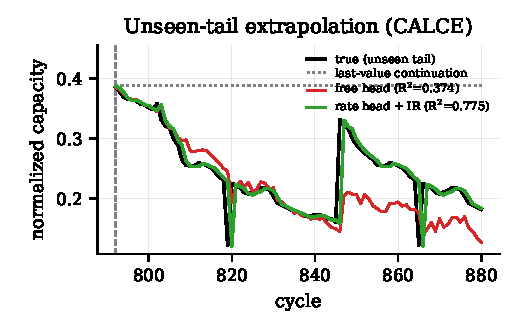
\includegraphics[width=\linewidth]{figures/fig_extrap}
\caption{Unseen-tail extrapolation on the CALCE test cell (train
90\%, evaluate the final 10\% right of the dashed line). Black: true
capacity; gray dotted: last-value continuation; red: main-model
readout; green: rate head + IR. The rate head continues the
degradation envelope instead of flattening or drifting.}
\label{fig:extrap}
\end{figure}

\begin{table}[htbp]
\centering
\caption{Unseen-tail extrapolation (train 90\%, evaluate final 10\%),
CALCE. Sliding-window protocol identical to the main results.}
\label{tab:extrap}
\footnotesize
\setlength{\tabcolsep}{3pt}
\begin{tabular}{lcc}
\toprule
Predictor & Tail R\textsuperscript{2} & Tail MAE (Ah) \\
\midrule
last-value continuation & $-5.28$ & 0.142 \\
main-model readout (free head) & 0.374 & 0.035 \\
\textbf{rate head + IR} & \textbf{0.7745$\pm$0.0001} & \textbf{0.0110$\pm$0.0001} \\
\bottomrule
\end{tabular}
\end{table}

\subsubsection{Corrupted-input robustness}

The capacity channel of the test sequence is corrupted (30\% packet
loss with hold-last-value, $\pm1\%$ Gaussian noise, 5\% impulse
glitches) while IR stays clean. This models a
capacity-channel-only failure (for example a current-sensor drift
or a capacity-estimator failure), in which the independently
measured impedance data remain valid; a total telemetry outage
affecting both channels is outside the scenario. The rate head wins
all four settings on every MAE contrast (clean $-34\%$, drop30
$-30\%$, gauss $-13\%$, impulse $-32\%$); under 30\% loss the
biased hold-last-value filling hurts the free head worst (MAE
$0.0104\pm0.0028$ vs.\ $0.0073\pm0.0010$; worst-case AE $574$
vs.\ $9$: the free head occasionally catastrophically misses the
crossing, while the rate head's AE stays bounded (median $1$ in
every mode). Figure~\ref{fig:robust} shows the
mechanism: the forward-filled input plateaus upward, dragging the
free head's near-EOL crossing late, while the rate head leans on the
clean IR channel and keeps the crossing close to truth. A caveat:
the IR signal strength varies across cells (correlation with
capacity $-0.98$ on CS2\_35/36/37 but only $-0.12$ on CS2\_38,
whose logged impedance is noisy), so the rate head's physics term
contributes where the IR measurement is informative; the learned
component must carry the fade otherwise.

\begin{figure*}[!t]
\centering

\includegraphics[width=\textwidth]{figures/fig_robust}
\caption{Drop30 corruption on the CALCE test cell. Left: full
trajectory (gray: corrupted forward-filled input; black: true; red:
free head, AE 23; green: rate head + IR, AE 17). Right: zoom on the
EOL-crossing region.}
\label{fig:robust}
\end{figure*}

\begin{table}[htbp]
\centering
\caption{Corrupted-input robustness (capacity channel corrupted, IR
clean), CALCE, ten seeds (mean $\pm$ std; AE as mean over seeds,
median 1 for the rate head in every mode).
$^{\dagger}$worst-case AE 574 in a single free-head seed;
$^{\ddagger}$worst-case AE 68 in a single rate-head seed.}
\label{tab:robust}
\scriptsize
\setlength{\tabcolsep}{3pt}
\begin{tabular}{lcc cc}
\toprule
Mode & \multicolumn{2}{c}{MAE (Ah)} & \multicolumn{2}{c}{AE} \\
 & free head & rate head & free head & rate head \\
\midrule
clean & $0.0065\pm0.0003$ & \textbf{$0.00424\pm0.00002$} & 1.9 & \textbf{1.0} \\
drop30 & $0.0104\pm0.0028$ & \textbf{$0.0073\pm0.0010$} & $59.6^{\dagger}$ & \textbf{3.4} \\
gauss ($\pm1\%$) & $0.0110\pm0.0005$ & \textbf{$0.0096\pm0.0003$} & 2.9 & \textbf{2.5} \\
impulse (5\%) & $0.0087\pm0.0003$ & \textbf{$0.0060\pm0.0001$} & \textbf{3.2} & $8.4^{\ddagger}$ \\
\bottomrule
\end{tabular}
\end{table}

\subsubsection{Interpretability of the rate head}

The rate head's physics-feature coefficient
$\operatorname{softplus}(\gamma)$ is non-negative by construction,
so the measured internal
resistance can only accelerate the predicted decay (the SEI-growth
direction), and the structural monotonicity removes nonphysical
regeneration artifacts (regen fraction $0.163$ vs $0.232$ for the
free head on CALCE). The learned rate component
$\operatorname{softplus}(\mathbf{w}^\top\mathbf{h})$ absorbs the
dataset-specific fade dynamics, leaving the IR term as an
interpretable, independently measured correction.

Figure~\ref{fig:stages} shows the coarse-branch pooled
representation of PANASONIC windows projected into two dimensions;
early/mid/late-life windows form separable clusters, confirming that
the coarse branch encodes the degradation stage ($93.2\%$ three-stage
linear separability).

\begin{figure*}[!t]
\centering
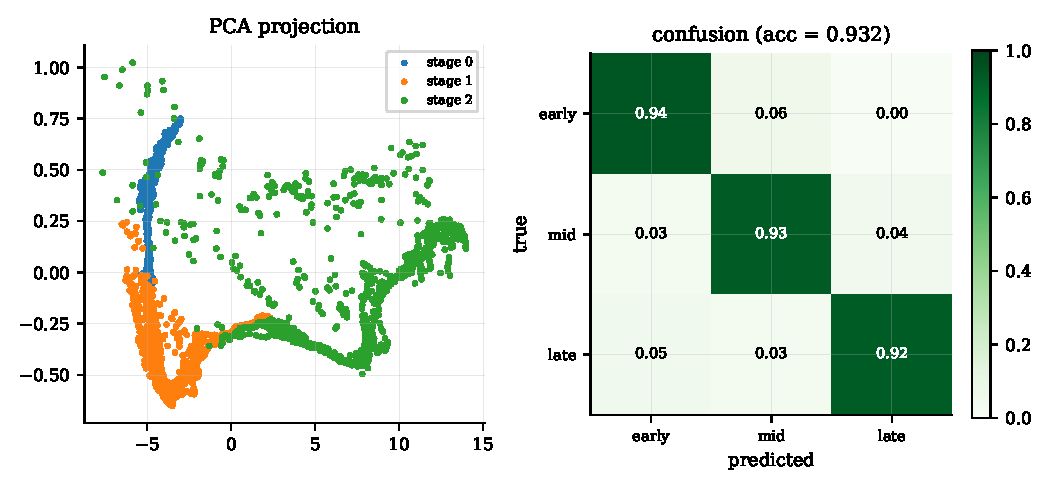
\includegraphics[width=\textwidth]{figures/fig_stages}
\caption{Coarse-branch (patch 8) pooled representations of
PANASONIC windows. Left: PCA projection colored by degradation
stage terciles; right: normalized three-stage confusion matrix of a
linear classifier on the projection (accuracy $93.2\%$).}
\label{fig:stages}
\end{figure*}

\subsection{Uncertainty quantification}
\label{sec:conf}

Table~\ref{tab:quantile} reports the quantile and conformal results on
CALCE. The P50 estimate matches the point model (MAE $0.0075\pm0.0007$ vs
$\approx 0.0074$). Raw pinball quantiles are miscalibrated: the P2.5--P97.5
interval covers only $89.1\%$ of observations against the nominal
$95\%$, a known failure mode of quantile regression under
distribution shift. Conformal calibration on a held-out cell
($n = 869$ windows) lifts coverage to
$93.5\%\pm0.9\%$ overall (ten training seeds, range
$91.9$--$95.1\%$), at a modest
$+36\%$ interval-width cost; the small residual gap to $95\%$
reflects finite-sample calibration ($n{=}869$) and cross-cell
distribution drift, and is reported honestly.
Figure~\ref{fig:uq_band} shows the calibrated band on the test cell.

\emph{From intervals to a decision rule.} The calibrated band
translates into an operational policy directly: the simplest
risk-aware rule is ``schedule replacement at the first cycle where
the P2.5 trajectory crosses the EOL threshold.'' With CQR the
$93.5\%\pm0.9\%$ coverage bounds the missed-EOL rate, and the
$+36\%$
interval-width cost quantified above is the price paid for that
bound. Quantifying the associated maintenance-cost trade-off under a
concrete cost model is left to future work.

\begin{figure}[htbp]
\centering
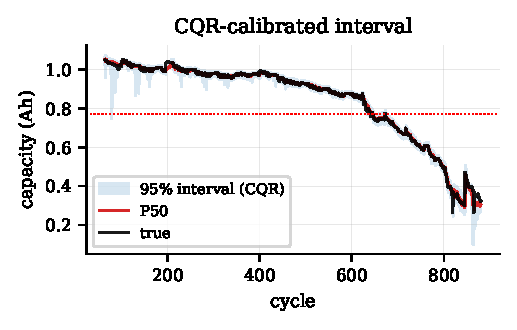
\includegraphics[width=\linewidth]{figures/fig_uq_band}
\caption{CQR-calibrated P2.5--P97.5 interval on the CALCE test cell
(shaded band), with the P50 trajectory and the measured capacity.
The interval is the deployment-ready output: one forward pass, two
calibration scalars, no ensemble.}
\label{fig:uq_band}
\end{figure}

\begin{table}[htbp]
\centering
\caption{Uncertainty quantification: pinball quantiles with
conformalized quantile regression (CQR), CALCE.}
\label{tab:quantile}
\footnotesize
\setlength{\tabcolsep}{3pt}
\begin{tabular}{lccc}
\toprule
Metric & Raw pinball & CQR & Target \\
\midrule
P50 MAE & 0.0075 & --- & $\approx$ point model (0.0074) \\
Coverage (overall) & 0.891 & 0.935 & 0.95 \\
Interval width & 0.0286 & 0.0421 & --- \\
\bottomrule
\multicolumn{4}{@{}p{\dimexpr\columnwidth-6pt\relax}@{}}{\footnotesize Ten seed-verified models (mean values; per-SP coverage is not broken out here -- the seed-to-seed spread 0.919--0.951 dominates the per-SP variation).}\\
\bottomrule
\end{tabular}
\end{table}

\subsection{Limitations}
\label{sec:limitations}

All main results are aggregated over ten training seeds per
starting point (seeds 1--10, per-SP protocol,
Table~\ref{tab:tableA}); the architecture ablation is PANASONIC-only,
under the same protocol and with parameter-matched arms, so it
isolates the cross-scale mechanism; the physics extension is also
ten-seed, and the
uncertainty study uses a
single calibration cell (CS2\_36), with its coverage verified over
ten training seeds ($93.5\%\pm0.9\%$). \emph{Epoch
sensitivity.} A continuation study on CALCE and NASA (ten seeds
per SP) probed the budget: extending every model from 100 to 200
epochs helps unevenly: NASA SP50 gains $19.6\%$ in MAE while SP70
and SP90 lose $2$--$4\%$, and the CALCE AE spread widens while its
MAE improves $1.5$--$7.9\%$. Extension to 300 epochs adds
nothing beyond noise. We therefore keep a \emph{uniform}
100-epoch budget for every dataset and variant, so all compared
models share one optimizer budget rather than a per-dataset one. The
official-style 0.8/0.2 row-tail early stopping was also tried; the
small validation window made it terminate at 2--16 epochs with
systematically worse test metrics, so the fixed schedule is kept.
All validation is on public laboratory cycling data;
field conditions such as partial cycling, pack-level effects, and
non-stationary loads remain open. The deployment chain is verified
separately, and the caveats that come with it are stated in
Section~\ref{sec:deploy}.

